\hypertarget{appendix-73c6b8ed5a87}{}
\section*{XR - Light, Vision and Perception - Visual Recall}
\section{Light, Vision and Perception --- Visual Recall}\label{appendix-73c6b8ed5a87-light-vision-and-perception-visual-recall}

\textbf{Scope:} Companion to \href{Continuous\%20Notes/University\%20-\%20Worlds,\%20Images\%20and\%20Inference\%20-\%20Graphics,\%20Vision\%20and\%20Photography}{Continuous Notes/University - Worlds, Images and Inference - Graphics, Vision and Photography}. This is a recall board: sketch the path, then explain what each stage measures and what it cannot establish.

\begin{quote}
{[}!abstract{]} One-page quick notes \textbf{Light → eye → task → display:} rendering is a loop; code values are not the light itself. \href{Continuous\%20Notes/University\%20-\%20Worlds,\%20Images\%20and\%20Inference\%20-\%20Graphics,\%20Vision\%20and\%20Photography\#Light\%20must\%20become\%20a\%20quantity\%20before\%20it\%20becomes\%20a\%20color}{Radiometry → colorimetry} \textbf{See only what survives the pipeline:} optics, contrast, adaptation, eccentricity, sampling and reconstruction all constrain visibility. \href{Continuous\%20Notes/University\%20-\%20Worlds,\%20Images\%20and\%20Inference\%20-\%20Graphics,\%20Vision\%20and\%20Photography\#The\%20eye\%20is\%20an\%20optical\%20instrument\%20with\%20neural\%20processing\%20inside\%20it}{Eye and neural processing} · \href{Continuous\%20Notes/University\%20-\%20Worlds,\%20Images\%20and\%20Inference\%20-\%20Graphics,\%20Vision\%20and\%20Photography\#Visibility\%20is\%20about\%20contrast,\%20conditions\%20and\%20tasks}{Visibility and task} \textbf{Time matters twice:} eye motion changes the retinal sample; history reuse predicts correspondence and must validate it. \href{Continuous\%20Notes/University\%20-\%20Worlds,\%20Images\%20and\%20Inference\%20-\%20Graphics,\%20Vision\%20and\%20Photography\#A\%20gaze\%20sample\%20needs\%20a\%20time\%20as\%20well\%20as\%20a\%20direction}{Gaze and time} · \href{Continuous\%20Notes/University\%20-\%20Worlds,\%20Images\%20and\%20Inference\%20-\%20Graphics,\%20Vision\%20and\%20Photography\#Temporal\%20reconstruction\%20is\%20an\%20inference\%20about\%20correspondence}{Temporal reuse} \textbf{Measure, don't assume:} quality metrics and thresholds answer only the question their procedure tested. \href{Continuous\%20Notes/University\%20-\%20Worlds,\%20Images\%20and\%20Inference\%20-\%20Graphics,\%20Vision\%20and\%20Photography\#Quality\%20numbers\%20need\%20a\%20question\%20they\%20can\%20actually\%20answer}{Quality metrics} · \href{Continuous\%20Notes/University\%20-\%20Worlds,\%20Images\%20and\%20Inference\%20-\%20Graphics,\%20Vision\%20and\%20Photography\#A\%20threshold\%20is\%20evidence\%20from\%20a\%20procedure,\%20not\%20a\%20universal\%20border}{Threshold evidence} \textbf{Spend detail where useful, safely:} foveation is a resource allocation with prediction uncertainty and latency margins. \href{Continuous\%20Notes/University\%20-\%20Worlds,\%20Images\%20and\%20Inference\%20-\%20Graphics,\%20Vision\%20and\%20Photography\#Foveation\%20is\%20allocation\%20under\%20uncertain\%20perception\%20and\%20timing}{Foveation}
\end{quote}

\subsection{Figure-linked short notes}\label{appendix-73c6b8ed5a87-figure-linked-short-notes}

Use one row at a time: explain the claim, open its figure, then follow the nearby chapter explanation. The figure labels are shared with the continuous chapter.

{\def\LTcaptype{none} % do not increment counter
\begin{longtable}[]{@{}
  >{\raggedright\arraybackslash}p{(\linewidth - 4\tabcolsep) * \real{0.3333}}
  >{\raggedright\arraybackslash}p{(\linewidth - 4\tabcolsep) * \real{0.3333}}
  >{\raggedright\arraybackslash}p{(\linewidth - 4\tabcolsep) * \real{0.3333}}@{}}
\toprule\noalign{}
\begin{minipage}[b]{\linewidth}\raggedright
Figure in the chapter
\end{minipage} & \begin{minipage}[b]{\linewidth}\raggedright
Shortest useful brief
\end{minipage} & \begin{minipage}[b]{\linewidth}\raggedright
Boundary to remember
\end{minipage} \\
\midrule\noalign{}
\endhead
\bottomrule\noalign{}
\endlastfoot
\href{Continuous\%20Notes/University\%20-\%20Worlds,\%20Images\%20and\%20Inference\%20-\%20Graphics,\%20Vision\%20and\%20Photography\#Figure\%20X0\%20—\%20A\%20qualitative\%20picture\%20of\%20the\%20XR\%20loop/}{X0 · Perception collage} & Scene → display light → optics → retina → task; gaze feeds rendering decisions. & Qualitative AI illustration; not calibrated rays or anatomical dimensions. \\
\href{Continuous\%20Notes/University\%20-\%20Worlds,\%20Images\%20and\%20Inference\%20-\%20Graphics,\%20Vision\%20and\%20Photography\#Figure\%20X1\%20—\%20Two\%20simultaneous\%20depth\%20demands/}{X1 · Focus and pointing} & Vergence points the eyes; accommodation changes focus. A near stereo target can coexist with a distant optical image. & Demanded distances can disagree; sharpness alone cannot fix that. \\
\href{Continuous\%20Notes/University\%20-\%20Worlds,\%20Images\%20and\%20Inference\%20-\%20Graphics,\%20Vision\%20and\%20Photography\#Figure\%20X2\%20—\%20The\%20samples\%20cannot\%20name\%20their\%20original/}{X2 · Aliasing witness} & At 10 Hz, 13 Hz and 3 Hz cosines give identical samples: their phase difference is whole cycles. & Filter before reducing sample rate; more bits cannot recover lost distinctions. \\
\href{Continuous\%20Notes/University\%20-\%20Worlds,\%20Images\%20and\%20Inference\%20-\%20Graphics,\%20Vision\%20and\%20Photography\#Figure\%20X3\%20—\%20Same\%20endpoints,\%20different\%20averaging\%20domain/}{X3 · Linear-light mean} & Black/white mean is 0.5 linear → about 0.73536 sRGB. Encoded mean 0.5 → about 0.21404 linear. & Values are normalized channels, not nits. Specify the encoding and arithmetic domain. \\
\href{Continuous\%20Notes/University\%20-\%20Worlds,\%20Images\%20and\%20Inference\%20-\%20Graphics,\%20Vision\%20and\%20Photography\#Figure\%20X4\%20—\%20Aim\%20detail\%20at\%20visible\%20time/}{X4 · Gaze timing} & Predict gaze for visible time; expand the sharp region for measured uncertainty. & A 90 Hz stream gives 11.11 ms intervals, not a latency measurement. \\
\end{longtable}
}

\textbf{Connect the rest:} \href{Continuous\%20Notes/University\%20-\%20Worlds,\%20Images\%20and\%20Inference\%20-\%20Graphics,\%20Vision\%20and\%20Photography\#Fourier\%20coordinates\%20reveal\%20what\%20a\%20filter\%20removes}{Fourier coefficients describe frequency and phase} · \href{Continuous\%20Notes/University\%20-\%20Worlds,\%20Images\%20and\%20Inference\%20-\%20Graphics,\%20Vision\%20and\%20Photography\#What\%20happens\%20to\%20a\%20point\%20of\%20light?}{PSF → OTF → MTF} · \href{Continuous\%20Notes/University\%20-\%20Worlds,\%20Images\%20and\%20Inference\%20-\%20Graphics,\%20Vision\%20and\%20Photography\#Temporal\%20reconstruction\%20is\%20an\%20inference\%20about\%20correspondence}{TAA requires valid correspondence} · \href{Continuous\%20Notes/University\%20-\%20Worlds,\%20Images\%20and\%20Inference\%20-\%20Graphics,\%20Vision\%20and\%20Photography\#A\%20threshold\%20is\%20evidence\%20from\%20a\%20procedure,\%20not\%20a\%20universal\%20border}{Thresholds depend on procedure} · \href{Continuous\%20Notes/University\%20-\%20Worlds,\%20Images\%20and\%20Inference\%20-\%20Graphics,\%20Vision\%20and\%20Photography\#Less\%20shading\%20does\%20not\%20mean\%20the\%20whole\%20frame\%20becomes\%20equally\%20faster}{Whole-frame savings need profiling}.

\subsection{Visual atlas --- what each view is for}\label{appendix-73c6b8ed5a87-visual-atlas-what-each-view-is-for}

\begin{figure}
\centering
\pandocbounded{\includegraphics[keepaspectratio,alt={Qualitative AI illustration of the XR perception loop, foveal and peripheral vision, and binocular focus cues.}]{xr_perception_pipeline.png}}
\caption{Qualitative AI illustration of the XR perception loop, foveal and peripheral vision, and binocular focus cues.}
\end{figure}

\emph{Illustration caption:} The rendered image is not the perceptual result. Light, optics, neural processing, task and display timing intervene. This is a qualitative AI teaching collage, not a calibrated optical ray diagram or anatomical measurement; \href{Continuous\%20Notes/University\%20-\%20Worlds,\%20Images\%20and\%20Inference\%20-\%20Graphics,\%20Vision\%20and\%20Photography\#Figure\%20X0\%20—\%20A\%20qualitative\%20picture\%20of\%20the\%20XR\%20loop}{open the same figure in context}.

{\def\LTcaptype{none} % do not increment counter
\begin{longtable}[]{@{}
  >{\raggedright\arraybackslash}p{(\linewidth - 4\tabcolsep) * \real{0.3333}}
  >{\raggedright\arraybackslash}p{(\linewidth - 4\tabcolsep) * \real{0.3333}}
  >{\raggedright\arraybackslash}p{(\linewidth - 4\tabcolsep) * \real{0.3333}}@{}}
\toprule\noalign{}
\begin{minipage}[b]{\linewidth}\raggedright
Recall figure
\end{minipage} & \begin{minipage}[b]{\linewidth}\raggedright
One-line takeaway
\end{minipage} & \begin{minipage}[b]{\linewidth}\raggedright
Open the full explanation
\end{minipage} \\
\midrule\noalign{}
\endhead
\bottomrule\noalign{}
\endlastfoot
\hyperref[appendix-73c6b8ed5a87-from-emitted-light-to-a-perceptual-claim]{Perception loop} & The display closes the loop by changing the next light reaching the observer. & \href{Continuous\%20Notes/University\%20-\%20Worlds,\%20Images\%20and\%20Inference\%20-\%20Graphics,\%20Vision\%20and\%20Photography\#Prologue\%20-\%20A\%20perfect\%20scene\%20can\%20still\%20make\%20a\%20poor\%20experience/}{Prologue} \\
\hyperref[appendix-73c6b8ed5a87-four-measurement-families-that-must-not-be-collapsed]{Measurement ladder} & Physical light, color matches, perception, metrics and experiments are different claims. & \href{Continuous\%20Notes/University\%20-\%20Worlds,\%20Images\%20and\%20Inference\%20-\%20Graphics,\%20Vision\%20and\%20Photography\#Light\%20must\%20become\%20a\%20quantity\%20before\%20it\%20becomes\%20a\%20color/}{Radiometry and colorimetry} \\
\hyperref[appendix-73c6b8ed5a87-sampling-and-filtering-preserve-what-can-be-distinguished]{Sampling loop} & Filter before sampling; reconstruction cannot recover distinctions already aliased. & \href{Continuous\%20Notes/University\%20-\%20Worlds,\%20Images\%20and\%20Inference\%20-\%20Graphics,\%20Vision\%20and\%20Photography\#Sampling\%20is\%20a\%20question\%20of\%20what\%20remains\%20distinguishable/}{Sampling and aliasing} · \href{Continuous\%20Notes/University\%20-\%20Worlds,\%20Images\%20and\%20Inference\%20-\%20Graphics,\%20Vision\%20and\%20Photography\#A\%20footprint\%20is\%20more\%20meaningful\%20than\%20an\%20isolated\%20pixel\%20center/}{Pixel footprint} \\
\hyperref[appendix-73c6b8ed5a87-temporal-reuse-is-a-correspondence-hypothesis]{History validation} & Reuse prior samples only when correspondence evidence supports them. & \href{Continuous\%20Notes/University\%20-\%20Worlds,\%20Images\%20and\%20Inference\%20-\%20Graphics,\%20Vision\%20and\%20Photography\#Temporal\%20reconstruction\%20is\%20an\%20inference\%20about\%20correspondence/}{Temporal reconstruction} \\
\hyperref[appendix-73c6b8ed5a87-foveation-is-a-budget-under-uncertainty]{Foveation margin} & Gaze prediction error and latency determine the safe high-detail region. & \href{Continuous\%20Notes/University\%20-\%20Worlds,\%20Images\%20and\%20Inference\%20-\%20Graphics,\%20Vision\%20and\%20Photography\#Foveation\%20is\%20allocation\%20under\%20uncertain\%20perception\%20and\%20timing/}{Foveation design} \\
\end{longtable}
}

\subsection{From emitted light to a perceptual claim}\label{appendix-73c6b8ed5a87-from-emitted-light-to-a-perceptual-claim}

\pandocbounded{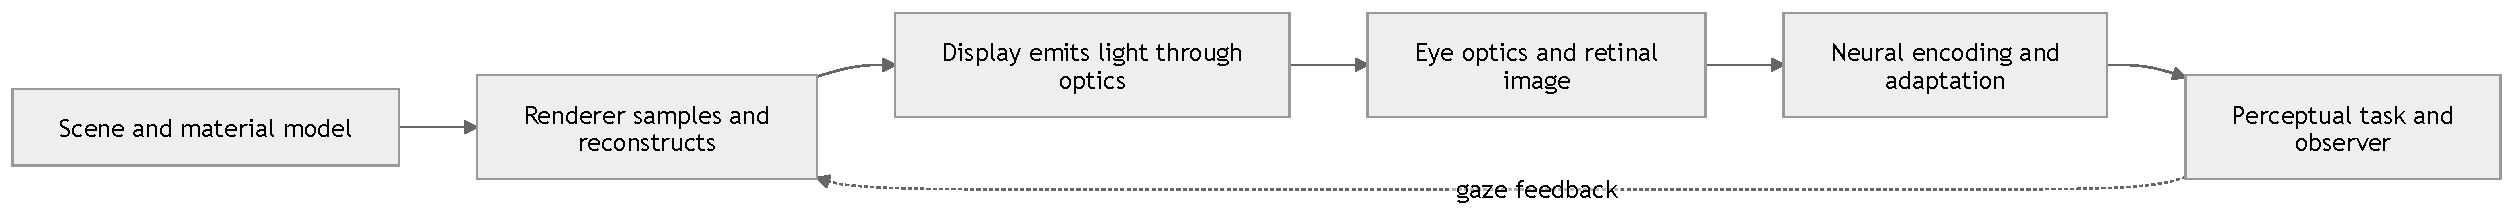
\includegraphics[keepaspectratio,alt={Diagram}]{../Assets/Print/16ca7fcd2c7b23b769dee3d080991551b90c772202e60d17ccffa485e4c0e589.pdf}}

\textbf{Caption:} The rendering loop is closed: the display changes the light reaching the observer, and observer/task conditions shape what counts as visible. RGB code values are not spectra and are not automatically linear-light energy.

\subsection{Four measurement families that must not be collapsed}\label{appendix-73c6b8ed5a87-four-measurement-families-that-must-not-be-collapsed}

\pandocbounded{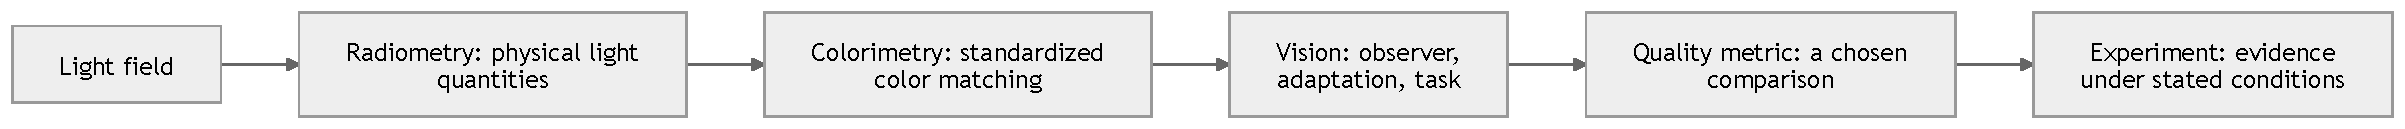
\includegraphics[keepaspectratio,alt={Diagram}]{../Assets/Print/1002cadfdb14972dd619f2ca5f4ae1972ddd227dc794b90983473a689f4bf874.pdf}}

\textbf{Caption:} A metric score is not a direct reading of human experience. Each transformation adds assumptions and conditions.

{\def\LTcaptype{none} % do not increment counter
\begin{longtable}[]{@{}
  >{\raggedright\arraybackslash}p{(\linewidth - 2\tabcolsep) * \real{0.5000}}
  >{\raggedright\arraybackslash}p{(\linewidth - 2\tabcolsep) * \real{0.5000}}@{}}
\toprule\noalign{}
\begin{minipage}[b]{\linewidth}\raggedright
Question
\end{minipage} & \begin{minipage}[b]{\linewidth}\raggedright
Distinction to retrieve
\end{minipage} \\
\midrule\noalign{}
\endhead
\bottomrule\noalign{}
\endlastfoot
How much physical light? & Radiant power/energy and radiance/irradiance are different quantities. \\
What color signal? & Spectrum and colorimetric coordinates are not interchangeable. \\
What does the eye resolve? & Acuity varies with eccentricity, contrast, adaptation and task. \\
Is the displayed result equivalent? & Focus/accommodation and binocular vergence can conflict in stereoscopic displays. \\
Does a score prove improvement? & Only for the metric, conditions, observers and task actually tested. \\
\end{longtable}
}

\subsection{Sampling and filtering: preserve what can be distinguished}\label{appendix-73c6b8ed5a87-sampling-and-filtering-preserve-what-can-be-distinguished}

\pandocbounded{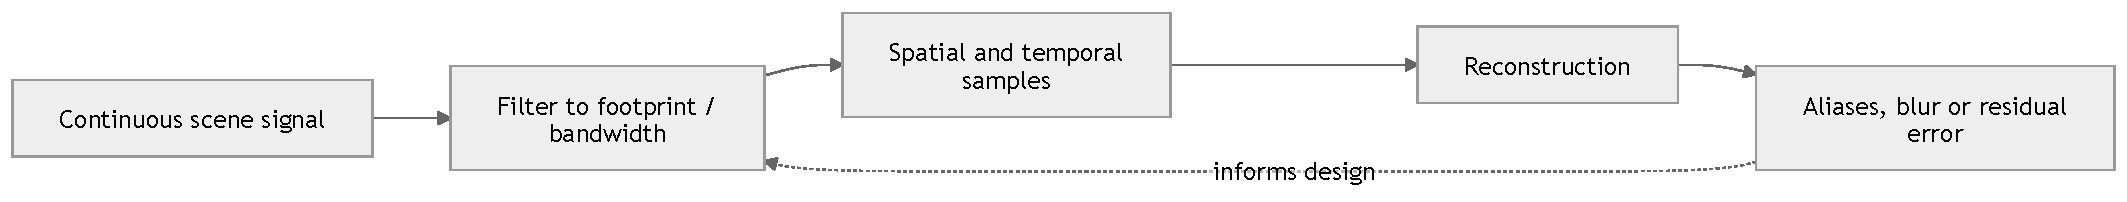
\includegraphics[keepaspectratio,alt={Diagram}]{../Assets/Print/9e4c98da2bb3ddb78e567bfb8dbbe9a0de1b0a1f242a8b77485add144402e864.pdf}}

\textbf{Caption:} Sampling without suitable filtering can make distinct signals produce identical samples. A pixel footprint, motion, and time interval all matter; one isolated pixel center is not a complete image measurement.

\subsection{Temporal reuse is a correspondence hypothesis}\label{appendix-73c6b8ed5a87-temporal-reuse-is-a-correspondence-hypothesis}

\pandocbounded{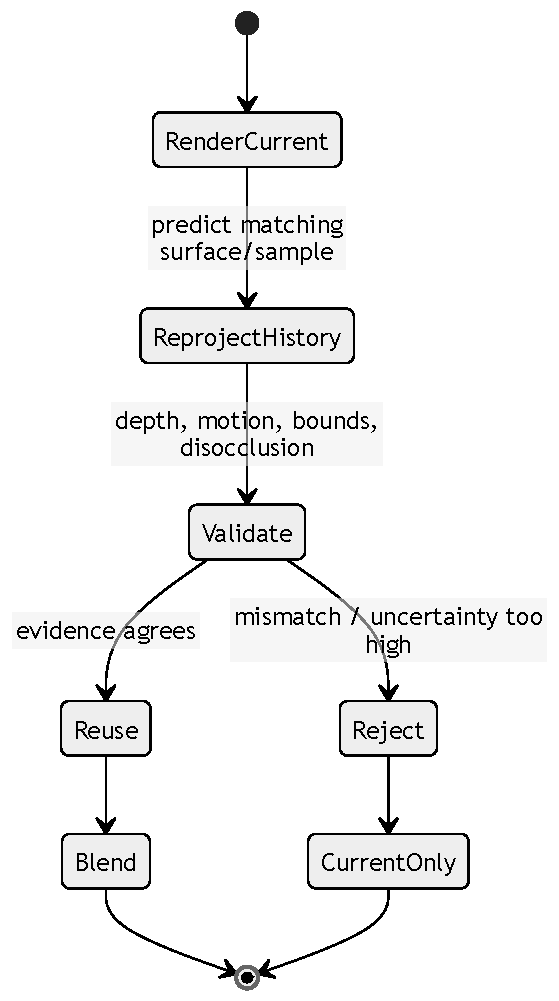
\includegraphics[keepaspectratio,alt={Diagram}]{../Assets/Print/682bff044b288d46f732759ae0c35312f3a9e6422575201da09dd2411070f283.pdf}}

\textbf{Caption:} Reprojection is not ``old pixels are correct.'' It is a prediction plus validation. Jitter, temporal antialiasing and motion blur address related but distinct problems.

\subsection{Foveation is a budget under uncertainty}\label{appendix-73c6b8ed5a87-foveation-is-a-budget-under-uncertainty}

\begin{verbatim}
gaze estimate ──> predicted gaze at display time ──> high-quality region
      │                        │                              │
      └── latency/error ───────┴── safety margin ────────────┘
                               ↓
                   lower peripheral work only where justified
\end{verbatim}

\textbf{Caption:} Less shading work does not imply the whole frame becomes equally faster. Prediction error, transition smoothness, display timing and workload determine the usable benefit.

\subsection{Retrieval prompts}\label{appendix-73c6b8ed5a87-retrieval-prompts}

\begin{enumerate}
\def\labelenumi{\arabic{enumi}.}
\tightlist
\item
  Why can two different continuous signals produce the same samples?
\item
  How do sampling rate, filter footprint and reconstruction relate?
\item
  What changes between linear-light averaging and averaging encoded RGB values?
\item
  Why can a sharp stereo image still feel uncomfortable?
\item
  What evidence is needed before a threshold can be treated as a boundary?
\item
  Why does valid foveation require a margin for gaze prediction error?
\end{enumerate}

\begin{quote}
{[}!answer{]}- Compact key Frequencies beyond the sampling system's distinguishable range can alias. Filtering limits content before discrete sampling; reconstruction defines what is inferred between samples. Nonlinear transfer encoding changes averages. Accommodation and vergence can demand different focal distances. A threshold depends on procedure and conditions, not just a fitted curve. Gaze latency/error can move the true fovea outside a region sized only around the estimate.
\end{quote}

\href{Continuous\%20Notes/University\%20-\%20Worlds,\%20Images\%20and\%20Inference\%20-\%20Graphics,\%20Vision\%20and\%20Photography\#Sampling\%20is\%20a\%20question\%20of\%20what\%20remains\%20distinguishable}{Teach the complete XR chapter} · \href{../01-Foundations-I/main.pdf\#nameddest=appendix-fd090d982a15-xr01---independent-seeing-and-representation-source}{Source ledger (01-Foundations-I, appendix-fd090d982a15-xr01-\/-\/-independent-seeing-and-representation-source)}
